\documentclass[12pt]{article}
\usepackage{amssymb}
\usepackage{amsmath}
\usepackage{tikz}
\usetikzlibrary{arrows, positioning}
\begin{document}
    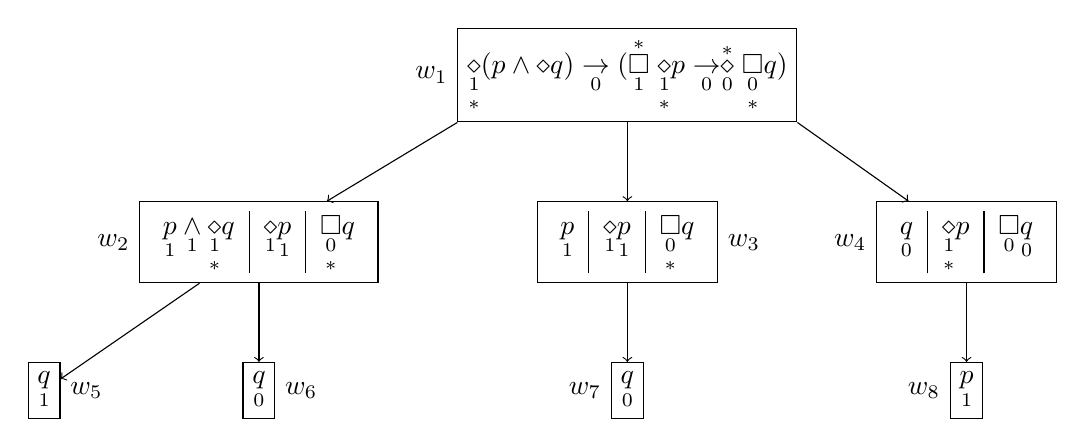
\begin{tikzpicture}[
    world/.style={rectangle,draw},
    invisible/.style={rectangle}]
        \node[world] (w_1)
            {$\underset{*}{\underset{1}{\diamond}} (p \land \diamond q)
              \underset{0}{\rightarrow}
              (\stackrel{*}{\underset{1}{\Box}} \underset{*}{\underset{1}{\diamond}} p
               \underset{0}{\rightarrow} \stackrel{*}{\underset{0}{\diamond}} \underset{*}{\underset{0}{\Box}} q)$
            };

        \node[black, left] at (w_1.west) {$w_1$};

        \node[world] (w_2) [below left=of w_1]
              {$\begin{array}{c|c|c}
                  \underset{1}{p} \underset{1}{\land} \underset{*}{\underset{1}{\diamond}} q &
                  \underset{1}{\diamond} \underset{1}{p} &
                  \underset{*}{\underset{0}{\Box}} q
              \end{array}$};

        \node[black, left] at (w_2.west) {$w_2$};

        \node[world] (w_3) [below=of w_1]
              {$\begin{array}{c|c|c}
                  \underset{1}{p} &
                  \underset{1}{\diamond}\underset{1}{p} &
                  \underset{*}{\underset{0}{\Box}} q
              \end{array}$};

        \node[black, right] at (w_3.east) {$w_3$};


        \node[world] (w_4) [below right=of w_1]
            {$\begin{array}{c|c|c}
                \underset{0}{q} &
                \underset{*}{\underset{1}{\diamond}} p &
                \underset{0}{\Box}\underset{0}{q}
            \end{array}$};

        \node[black, left] at (w_4.west) {$w_4$};


        \node[world] (w_5) [below left=of w_2]
              {$\underset{1}{q}$};

        \node[black, right] at (w_5.east) {$w_5$};

        \node[world] (w_6) [below=of w_2]
              {$\underset{0}{q}$};

        \node[black, right] at (w_6.east) {$w_6$};

        \node[world] (w_7) [below=of w_3]
             {$\underset{0}{q}$};

        \node[black, left] at (w_7.west) {$w_7$};

        \node[world] (w_8) [below=of w_4]
             {$\underset{1}{p}$};

        \node[black, left] at (w_8.west) {$w_8$};

        \draw[->] (w_1.south west) -- (w_2);
        \draw[->] (w_1.south) -- (w_3);
        \draw[->] (w_1.south east) -- (w_4);

        \draw[->] (w_2) -- (w_5);
        \draw[->] (w_2) -- (w_6);

        \draw[->] (w_3) -- (w_7);

        \draw[->] (w_4) -- (w_8);


         % \draw[->] (w_1) to[bend left = 30] (w_2.east);
         % \draw[->] (w_1) to[bend right = 20] (w_3.west);

         % \draw[->] (w_1) to[bend left = 20] (w_4.east);
         % \draw[->] (w_2) -- (w_4);
         % \draw[->] (w_4) -- (w_2);

         % \draw[->] (w_1) to[bend right = 20] (w_5.west);
         % \draw[->] (w_3) -- (w_5);
         % \draw[->] (w_5) -- (w_3);


    \end{tikzpicture}
\end{document}
